\documentclass[12pt]{article}
\linespread{1.1}
\usepackage[margin=1in]{geometry}
\usepackage{amsmath}
\usepackage{booktabs}
\usepackage{listings}
\usepackage{algorithm2e}
\usepackage{appendix}
\usepackage{wrapfig}
\usepackage{epsfig}
\usepackage{float}
\usepackage{palatino,mathpazo,inconsolata}
\usepackage{graphicx}
\usepackage{fancyhdr}
\usepackage{hyperref}

\pagestyle{fancy}
\lhead{Rivera and Chen}
\rhead{Numerical Exploration of Local Volatility}


\usepackage[dvipsnames]{xcolor}
\definecolor{lgray}{gray}{0.95}
\definecolor{mygreen}{rgb}{0,0.6,0}
\definecolor{mygray}{rgb}{0.5,0.5,0.5}
\definecolor{mymauve}{rgb}{0.58,0,0.82}

\hypersetup{
    colorlinks = true,
	  linkcolor = RoyalBlue,
    urlcolor = blue,
    citecolor = Blue
}

\numberwithin{equation}{section}

\lstset{
  backgroundcolor=\color{lgray},  
  basicstyle=\ttfamily\scriptsize,       
  breakatwhitespace=true,        
  breaklines=true,                
  commentstyle=\color{mygreen},   
  deletekeywords={...},           
  escapeinside={\%*}{*)},         
  extendedchars=true,             
  keepspaces=true,                
  keywordstyle=\color{blue},      
  language=Python,                
  morekeywords={*,...},           
  numbers=left,                   
  numbersep=5pt,                  
  numberstyle=\tiny\color{mygray},
  rulecolor=\color{black},        
  showspaces=false,               
  showstringspaces=false,         
  showtabs=false,                 
  stepnumber=1,                   
  stringstyle=\color{mymauve},    
  tabsize=2,	                  
  columns=fullflexible
}



\newcommand{\diff}[2]{\frac{\partial #1}{\partial #2}}
\newcommand{\Norm}{\mathcal N}
\newcommand{\abs}[1]{\left|#1\right|}
\newcommand{\norm}[1]{||#1||}
\newcommand{\pr}[1]{\left(#1\right)}
\usepackage{natbib}

\begin{document}

\onecolumn

\title{A Numerical Exploration of the Local Volatility Model for Option Pricing}
\author{Francisco Rivera \and Kevin Chen}
\date{\today}

\maketitle

\begin{abstract}
In Nobel-prize winning work, Black, Merton, and Scholes developed a model to
price options. The tractability of the model revolutionized options pricing and
allowed for the derivatives to become widely traded. However, the
predictions of the model run counterfactual to empirically observed prices. In
this paper, we consider a generalization to the Black-Scholes model, the
local-volatility model. This generalization gives us more degrees of freedom to
fit the prices we observe. With the additional expressiveness, however, come
numerical complications. Black-Scholes requires fitting only a single number
known as the \emph{implied volatility}, but the local volatility model requires
fitting an entire multi-dimensional function. We explore these complications and
arrive at solutions that are assessed for numerical stability and accuracy to
price out-of-sample options.
\end{abstract}

\tableofcontents

\newpage

\section{Background}
\label{sec:background}

\subsection{Options Terminology}
\label{subsec:terminology}

Before delving into the theoretical and numerical results, we briefly summarize
options terminology. An option is a \emph{derivative} on some asset, henceforth called
the \emph{underlying}---i.e.\ it's value is \emph{derived} from the value of the
underlying. The owner of a call (resp. put) option has the right but not the obligation
to buy (resp. sell) the underlying asset at a given price at some date in the future.

The price at which the holder of the option can buy/sell is called the
\emph{strike price}, denoted $K$. Invoking the right to buy or sell is called
\emph{exercising} the option. The last time at which the holder can exercise is
called the \emph{expiry}, denoted as time $T$. The value of the underlying asset
at time $t$ is denoted as $S_t$ (and sometimes the subscript is dropped whenever
it is implied). 

The payoff of a call option at expiry is thus given by,
\begin{equation}
 \max(S_T - K, 0) 
\label{eqn:callpayoff}
\end{equation}
because the owner will only exercise it if the underlying is worth more than the
strike price. This function gives rise the characteristic ``hockey-stick''
payoff diagram of an option at expiry,

\begin{center}
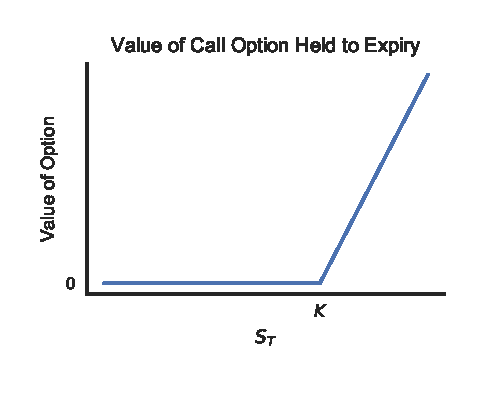
\includegraphics{figs/calloptpayoff}
\end{center}

The payoff of a put option is very similar to equation \ref{eqn:callpayoff},
\begin{equation}
 \max(K-S_T, 0) 
\end{equation}
because the owner of the option will only exercise it if the underlying is worth
less than the strike price, 
and the payoff curve looks like its mirror image,

\begin{center}
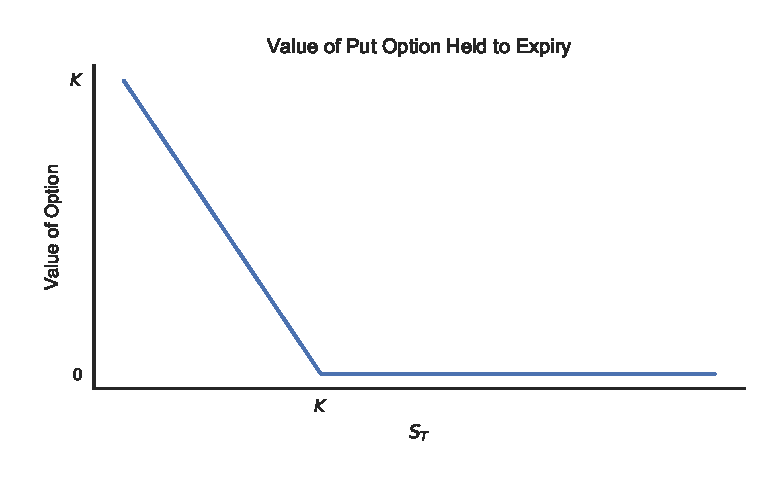
\includegraphics{figs/putoptpayoff}
\end{center}

\subsection{Risk-Neutral Pricing}
\label{subsec:riskneutral}

The value of an option at expiry is easily observable and displayed in the
figures in Section \ref{subsec:terminology}. However, before time $T$, the
value of $S_T$ is a random variable. Asset pricing (change of measure) 
%TODO add citation
theorems
allow us to write the value of a call option as the discounted expectation of
the payoff under what we call the \emph{risk-neutral distribution},
\begin{equation}
 \frac{C(S_0, K, T)}{e^{-rT}} = \int_K^\infty (S - K)
\underbrace{\phi(S, T; S_0)}_\text{risk-neutral PDF} \, dS
\label{eqn:riskneutralpricing}
\end{equation}
However, in order to make any progress beyond this, we need to make a further
assumption about what this risk-neutral distribution looks like.

\subsection{Black-Scholes Model}
\label{subsec:bs}
The Black-Scholes model makes one such assumption by writing how the asset
diffuses over time. In particular, the Black-Scholes model treates the asset
price as a geometric Brownian motion represented by the following stochastic difference equation:
\begin{equation}
 \frac{dS}{S} = r dt + \sigma dW 
\end{equation}
where $W$ is Brownian motion and $\sigma$ is a constant value called the \emph{implied
volatility}. 

This forces the risk-neutral distribution to be log-normal and makes
finding the price analytically tractable. In particular, since the only pricing
input into this model that we do not observe is the implied volatility, we can
quote price as a function of implied volatility (e.g. an option is said to cost
$\sigma=16\%$ if its price is consistent with the price the Black-Scholes model
would predict if $\sigma=16\%$).

Thus, Black-Scholes predicts that if $\sigma$ is indeed a constant, then for any
option written on the same underlying (regardless of strike price or expiry),
that the implied volatility will be (approximately) constant. However, this is
directly counterfactual to the options prices that we observe. For example,
looking at the prices of AAPL options that expire on April 2018 retrieved on
December 17$^\text{th}$, 2017 from Yahoo Finance, we get the following curve

\begin{center}
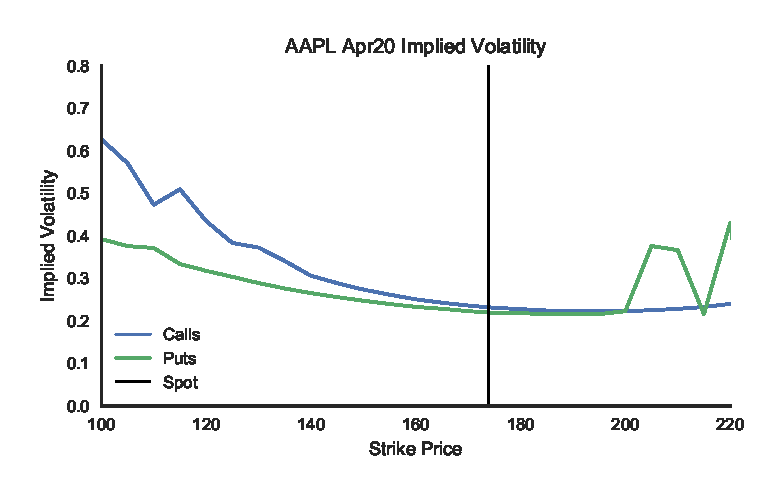
\includegraphics{figs/aapliv}
\end{center}

While the data is noisy, particularly for deep-in-the money\footnote{A call
(resp. put) option is said to be \emph{in-the-money} when $S_0 > K$ (resp. $S_0
< K$), \emph{out-of-the-money} when $S_0 < K$ (resp. $S_0 > K$), and at the
money if $S_0 = K$.} puts which are hardly ever traded, the graph is
unmistakably not constant. Moreover, AAPL is not an exception: most graphs of
implied volatility versus strike have a similar shape. These deviations from
Black-Scholes also correspond to intuitive qualitative ideas. If the price of
AAPL has just plunged 50\%, it is palatable to think there is a lot of investor
uncertainty, and that the future price of AAPL will diffuse with higher
volatility than if it is just up 5\%.  Thus, the assumption of constant $\sigma$
is suspect.

\section{Local Volatility Theory}
\label{sec:localvoltheory}

The \emph{local-volatility model} directly responds this shortcoming of the
Black-Scholes model by rewriting the diffusion equation as,
\begin{equation}
 \frac{dS}{S} = r dt + \sigma(S,t) dW 
\end{equation}
such that the volatility is no longer a global constant, but rather a function
of spot-price and time. We refer to this function as the \emph{local volatility
function}, and the value of the function at any given point as the \emph{local
volatility}. Note of course that in the special case when $\sigma$ is a constant
function, we have simply recovered the Black-Scholes model. We will make use of
this fact when we need to confirm the numerical results of the local volatility
model against theoretical closed-forms.

In the general case, though, we care about what the local volatility surface
says about prices and vice-versa. To this end, we can invoke Dupire's\footnote{
TODO: citation needed} work. The first thing to note is that we can
differentiate our risk-neutral pricing formula with respect to $K$ twice to get
that,
\begin{equation}
 e^{-rT} \phi(K, T; S_0) = \frac{\partial^2 C}{\partial K^2}.
\end{equation}
Moreover, because we have a diffusion rule for the underlying $S_t$, the
probability distributions must satisfy 
the \emph{Fokker-Planck equation}. 
%TODO: move the parenthetical to a footnote
%TODO: Add citation
(We
display this without drift. In practice, we can do this for the underlying
itself if is driftless, but if we are worried about drift, we can simply use the
forward price which is by construction a martingale),
\begin{equation}
 \frac{\partial C}{\partial T} = \frac{1}{2} e^{rT} \sigma^2 K^2 \frac{\partial^2
C}{\partial K^2}
\end{equation}
Rearranging gives us Dupire's equation,
\begin{equation}
 \sigma^2(K, T, S_0) = \frac{ \frac{\partial C}{\partial T} e^{-rT}}
{\frac{1}{2} K^2 \frac{\partial^2 C}{\partial K^2}}.
\end{equation}
We can also rewrite this assuming 0 interest rates, which we will assume going
forward for simplicity,
\begin{equation}
 \sigma^2(K, T, S_0) = \frac{ \frac{\partial C}{\partial T}}
{\frac{1}{2} K^2 \frac{\partial^2 C}{\partial K^2}}.
\end{equation}

There are a couple notable takeaways from this equation. First of all, if we
fully and perfectly observed a continuum of option prices for all strikes and
expiries, we would be able to uniquely determine the local volatility surface.
Moreover, we can do this \emph{regardless} of what the option prices
are\footnote{We get negative local volatility if arbitrage conditions are violated,
but we assume this does not happen.}. This means that unlike Black-Scholes, the
local volatility model can perfectly fit what we see, and we should be
apprehensive of overfitting.


\section{Pricing with Local Volatility}
\label{sec:localvolpricing}

In this section, we will concern ourselves with what we can do once we have the
local volatility surface. In particular, our main objective will be to 
price options. Note that the prices may exist in the market (e.g.\ as a sanity
check for our model), or they may not (e.g.\ to price options with expiries that
are not quoted, giving our model predictive power).

\subsection{Monte-Carlo Methods}
\label{subsec:montecarlopricing}

One way to do this is by realizing that the price is an expectation under the
risk-neutral distribution of the pay-off random variable (as in Equation
\ref{eqn:riskneutralpricing}). Thus, if we can sample
from this distribution, we can invoke the law of large numbers and get an
estimate for its average with sufficient samples. To this end, first we build a
function that allows us to sample from the risk-neutral distribution of ending
spot prices in Listing \ref{lst:sampleendprice}.

In this implementation, we have two types of numerical error to reason about.
The first is simply sampling error. Because we are only taking a finitely many
number of draws from the distribution, our sample mean will differ from the true
mean by a quantity that decreases with $\sqrt{n}$. Harder to reason about is the
discretization error that we introduce. 

% TODO: what is the discretization error of this? Can we assess it theoretically
% (if not, we can surely reason about it empirically by seeing how different
%  values we get for different number of discretization intervals are, though
%  this may prove tricky if the sampling error requires us to run an
%  unreasonable number of samples for each number of intervals)


\subsection{Discretization errors in Monte Carlo pricing}
In Monte Carlo pricing, we draw from the distribution of $S_T$ and compute option prices. We start with the stochastic difference equation\footnote{We assume interest rates are zero, and so there is no drift term for simplicity} \[
dS_t = S_t \sigma(S_t,t) \, dW_t,
\]
and approximate with finite differences 
\begin{equation}
    \label{eq:euler-maruyama}
    \tilde S_{t_{k+1}} - \tilde S_{t_k} = \tilde S_{t_k} \sigma(\tilde S_{t_k}, t_k)\, (W_{t_{k+1}} - W_{t_k}) = \tilde S_{t_k} \sigma(\tilde S_{t_k}, t_k) \sqrt{t_{k+1}-t_k} Z_k,
\end{equation}
for some $Z_k = \frac{W_{t_{k+1}} - W_{t_k}}{\sqrt{t_{k+1}-t_k}} \sim \Norm(0,1)$. This is the well-known \emph{Euler-Maruyama method}, an extension of the forward Euler method in stochastic calculus. It has been shown that the recursively-computed sequence $\tilde S_{t_1},\ldots, \tilde S_{t_N}$ converges to a draw from the true stochastic process $S_t$ as the mesh of the partition $\{t_1,\ldots,t_N\}$ tends to zero \citep{dobrow2016introduction}.  

Moreover, we can bound the rate of convergence. Let $\Delta t = t_{k+1} - t_k$ and suppose that $S_{t_k}$ is a draw from the true distribution. Let $S_{t_{k+1}}$ be drawn from the true distribution conditional on $S_{t_k}$, and let $\tilde S_{t_{k+1}}$ be the corresponding finite difference approximation via \eqref{eq:euler-maruyama} with respect to the same draw from the Brownian motion $W_t$. We have the following bounds on convergence \citep{higham2001algorithmic}: \begin{align}
E\abs{S_{t_{k+1}} - \tilde S_{t_{k+1}}} &\le C_1(\Delta t)^{1/2} \tag{Strong convergence} \\
\abs{E(g(\tilde S_{t_{k+1}})) - E (g(S_{t_{k+1}}))} &\le C_2 \Delta t \tag{Weak convergence}
\end{align}
for a $g$ that satisfies certain regularity conditions. 
Applying an equally-spaced partition to $[0,T]$ with step-size $\Delta t$, we immediately observe that the draws from the distribution at expiry must obey the same bounds of convergence: \begin{align*}
E\abs{S_{T} - \tilde S_{T}} &= O\pr{(\Delta t)^{1/2}} \\
\abs{E(g(\tilde S_{{T}})) - E (g(S_{T}))} &= O(\Delta t).
\end{align*}
Since we apply Euler-Murayama method to option pricing, we are more interested in the error $\abs{E(g(\tilde S_T)) - E(g(S_T))},$ where $g$ is a function of the form $g(S_T) = \max(S_T - K, 0)$ (for call options). The nondifferentiability of $g$ may pose some concern, as \cite{higham2001algorithmic} notes that the weak convergence bound works for $g$ smooth. However, since there exists a sequence of smooth functions $\tilde g$ that uniformly converges to $g(S_T) = \max(S_T - K, 0)$, we have \[
\abs{E(g(\tilde S_T)) - E(g(S_T))} \le 2\norm{g-\tilde g}_\infty + \abs{E(\tilde g(\tilde S_{{T}})) - E (\tilde g(S_{T}))},
\]
where $\norm{g-\tilde g}_\infty$ can be arbitrarily small. 
\section{Fitting Local Volatility}
\label{sec:localvolfitting}


\section{Theoretical analysis of numerical methods}
\label{sec:theory}
Our approach involves two separate applications of numerical techniques. First, we observe existing option prices $C(K,T)$ and compute the local volatility function via Dupire's equation \[
\sigma^2 = \frac{\diff{C}{T}}{\frac{1}{2}K^2\diff{^2C}{K^2}}.
\] 
Second, given an estimate of the local volatility $\sigma^2$, we numerically predict option prices. In this section, we discuss some theoretical difficulties in deriving analytical bounds on our approximations. In particular, we proceed in reverse order. We first discuss the numerical errors of Monte Carlo pricing, assuming the local volatility $\sigma^2$ is known.


\paragraph{Numerical experiment of first-order convergence of discretization error} Let $S_0 = 1, K = 1.1$, and \[\sigma(S, t) = \min\pr{0.1 + (S - 1)^2, 0.5}.\] Consider a call option at expiry $T = 1$ with strike $K$, whose payoff is $\max(S_T, K) - K$. Assume zero interest rate. We approximate the expectation with sample mean with sample size $10^6$. We approximate the true value of the option by computing the Euler-Murayama approximation with step-size equalling $1/200$. We then plot the pricing errors of Euler-Murayama approximations with step size $1/n$ for $n=1,\ldots,40$ in Figure~\ref{fig:log-log}. 
\begin{figure}[h!]
    \centering
    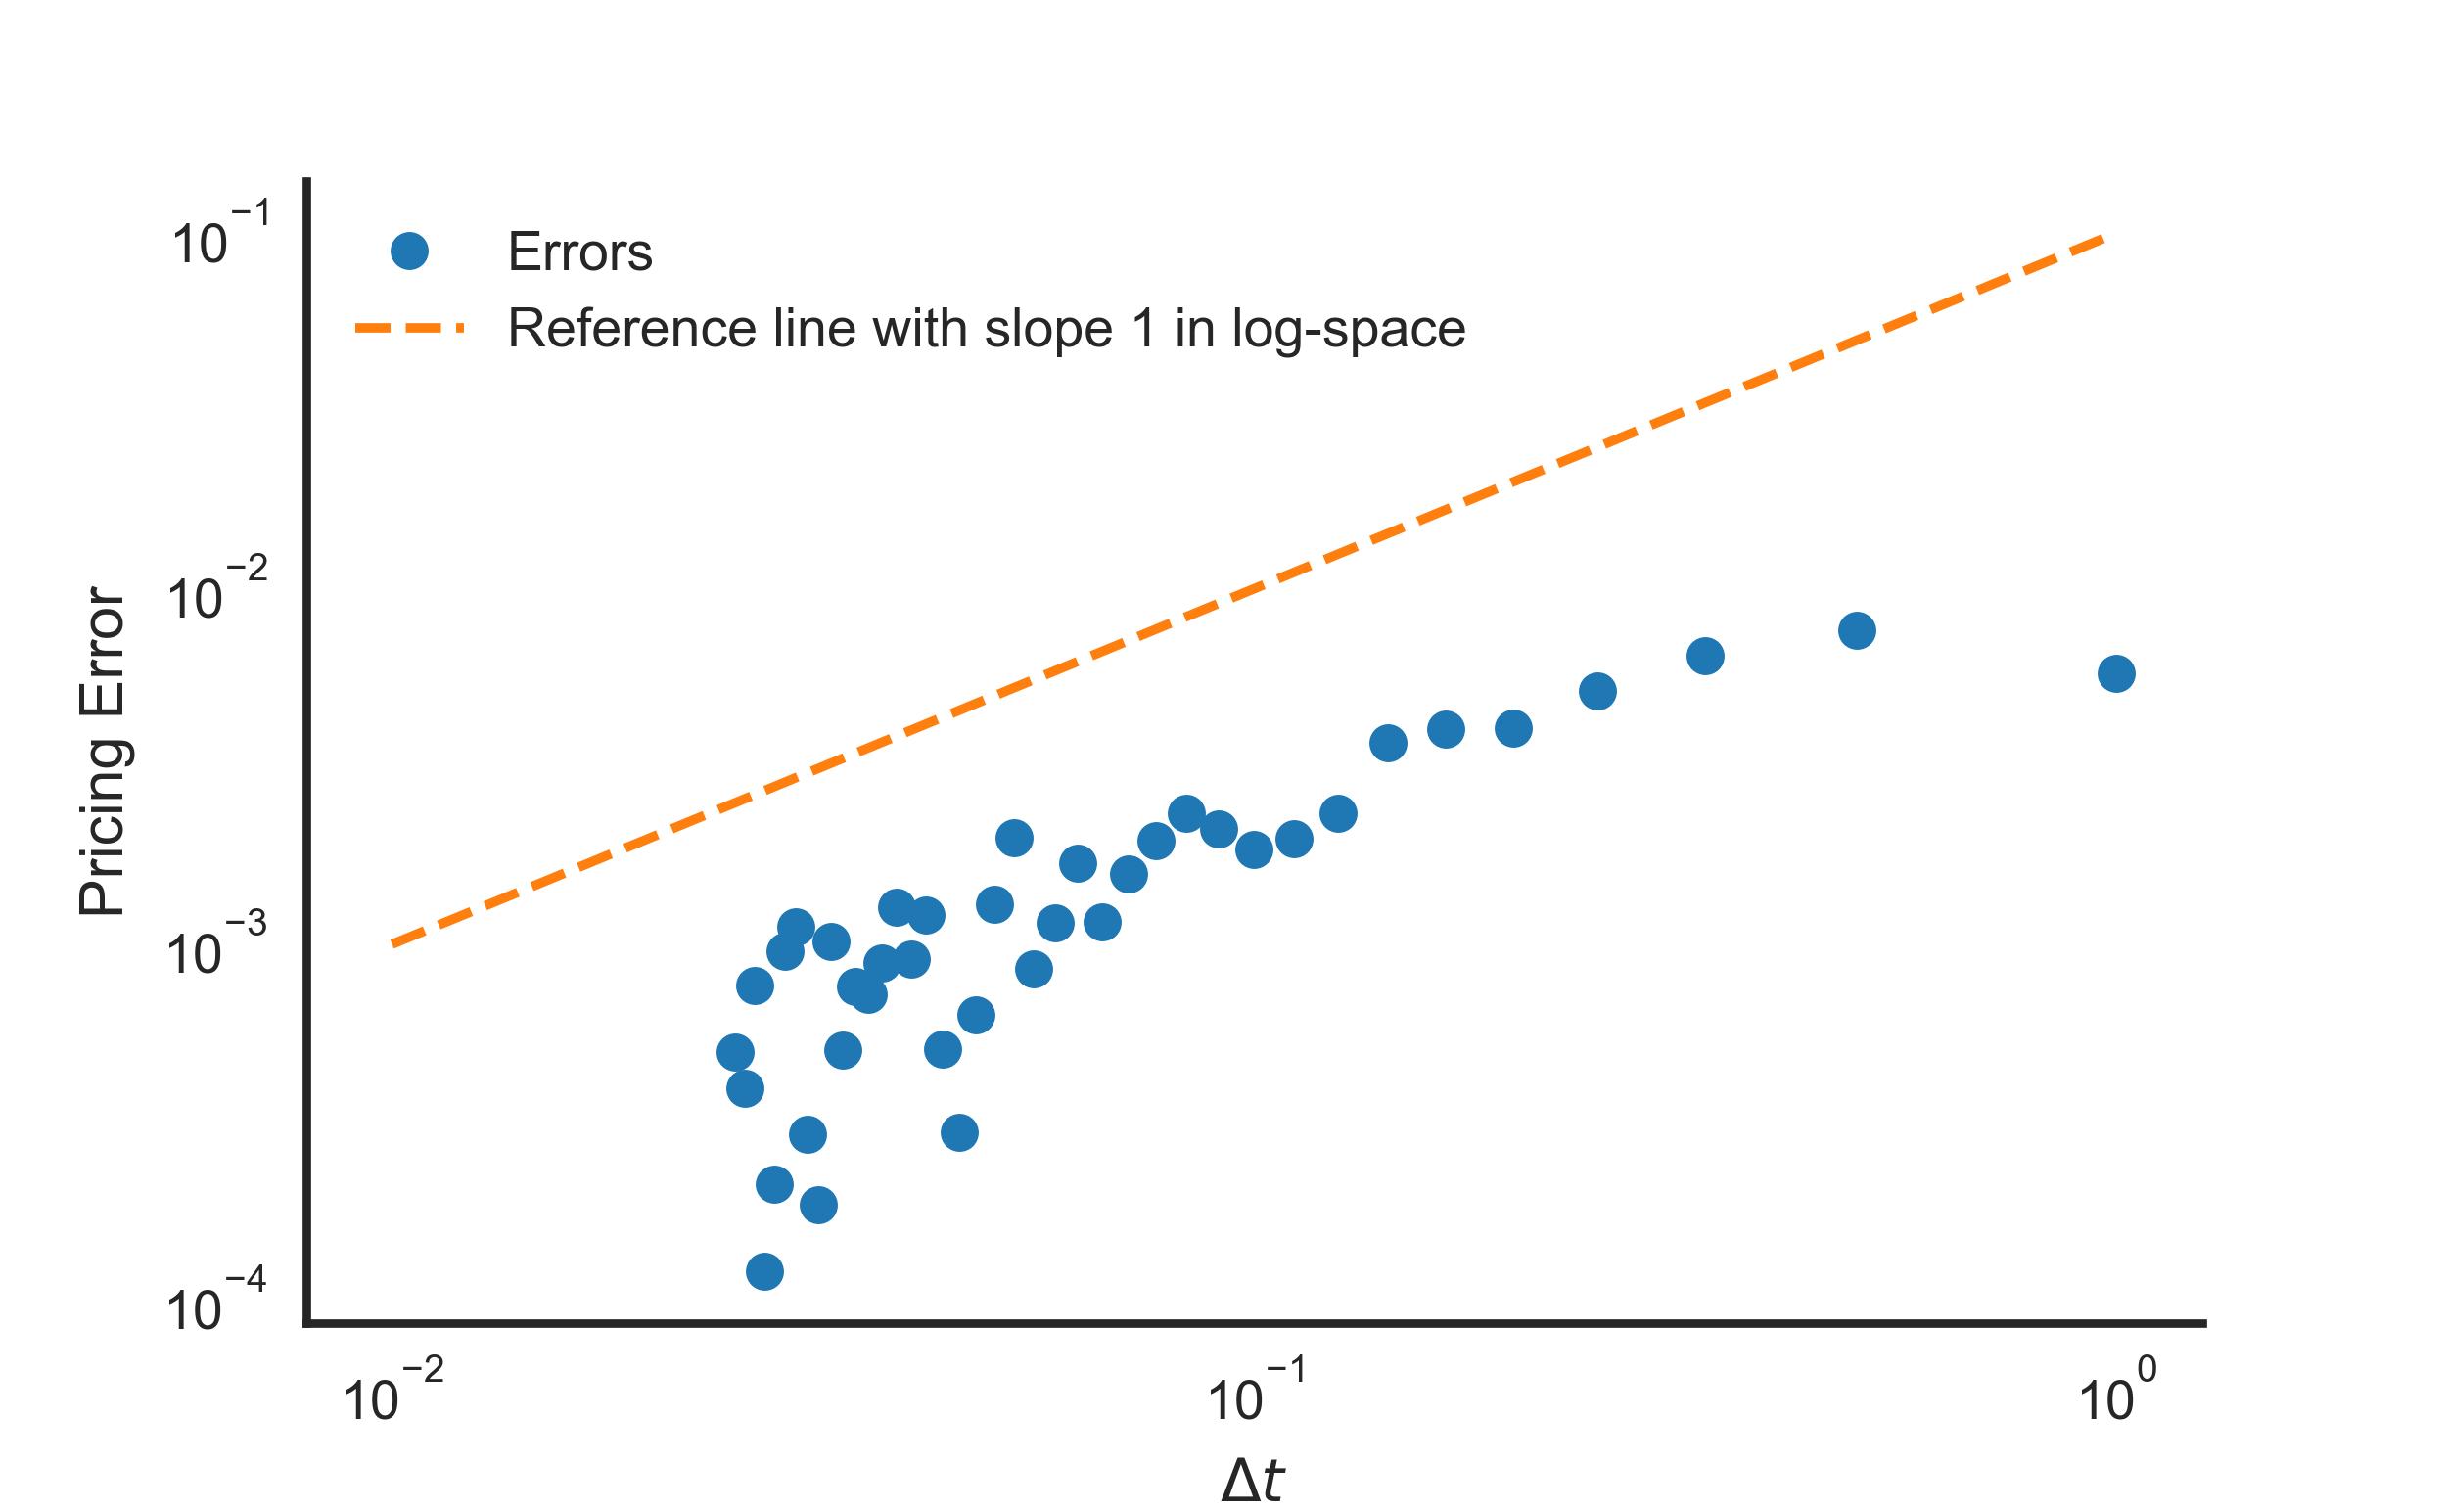
\includegraphics[width=0.5\textwidth]{figs/montecarlo_discrete.png}
    \caption{Log-log plot of pricing error against $\Delta t$}
    \label{fig:log-log}
\end{figure}
It is difficult to control the Monte Carlo sampling error, due to computational resource constraints, but we do observe approximately a first-order convergence pattern. 


Thus, for a known $\sigma^2$, we can limit the size of the discretization error at rate $O(\Delta t)$, and the size of the sampling error at rate $O(n^{-1/2})$ where $n$ is the sample size. The theory and the numerical experimentation suggests that the Monte Carlo pricing method is numerically robust. 
\subsection{Approximation of Dupire's equation}
However, computing $\sigma^2$ from observed data accurately is a much more difficult task. We illustrate the main difficulty below.

Let $A = \diff{C}{T} + e_1$ and $B = \diff{^2C}{K^2} + e_2$ be two approximations. Then \[
\frac{A}{\frac{1}{2}K^2 B} = \sigma^2 \frac{\diff{^2C}{K^2}}{\diff{^2C}{K^2} + e_2} + \frac{e_1}{\frac{1}{2}K^2 B}.
\]
Thus the absolute error \[
\abs{\frac{A}{\frac{1}{2}K^2 B} - \sigma^2} \le \sigma^2 \abs{\frac{e_2}{\diff{^2C}{K^2}+e_2}} + \abs{\frac{e_1}{\frac{1}{2}K^2B}}.
\]
Since $\diff{^2C}{K^2} > 0$, it should be unsurprising that the error vanishes as $e_1,e_2 \to 0$. However, note that deep-in-the-money options are virtually indistinguishable from the underlying asset, whereas deep-out-of-the-money options are virtually worthless. Thus $C$ is almost linear as a function of $K$ when $K$ is away from $S_0$.
%TODO: figure
Even though $\diff{^2C}{K^2} > 0$, the infimum of this second derivative is zero. This presents a first difficulty when attempting to bound the error of the approximations. A second challenge arises from the discreteness of empirical prices. We cannot evaluate the function $C(K,T)$ anywhere we wish, but rather we only observe its values on a grid whose fineness is capped at the finest intervals that prices are quoted in. To make matters worse, the prices quoted are accurate to $\$0.01$, and so it is as if we are working in a world where machine precision is nontrivially large.


The usual centered difference approximations have \[
|e_1|\le \frac{h_1^2}{6}\sup \abs{\diff{^3C}{T^3}} + \frac{\epsilon}{2h_1} \qquad |e_2| \le \frac{h_2^2}{12}\sup \abs{\diff{^4C}{K^4}} + \frac{2\epsilon}{h_2^2}.
\]
For values of $\diff{^2C}{K^2}$ sufficiently large, it is plausible that these approximations are sufficiently accurate. However, the approximation is certainly not accurate for values of $\diff{^2C}{K^2}$ close to zero. Yet for these values, which correspond to deep-money options, the option price is virtually known---the large errors in $\sigma^2$ for $K$ far away from $S_0$ is weighted by the extremely small probability that such errors matter. Such weighting is analytically intractable, and we mainly focus on numerical experimentation. 


\section{Conclusions}

\bibliographystyle{chicago}
\bibliography{am205.bib}

\newpage

\appendix
\appendixpage

\section{Code}

\lstinputlisting[
    caption=Sampling from risk-neutral $S_T$ distribution,
    label=lst:sampleendprice]{scripts/sampleendprice.py}

\lstinputlisting[
    caption=Pricing call option from Monte-Carlo samples,
    label=lst:pricecall]{scripts/pricecall.py}

\lstinputlisting[
    caption=Price using Black-Scholes formula,
    label=lst:blackscholesprice]{scripts/blackscholesprice.py}

\end{document}
